%%%%%%%%%%%%%%%%%%%%%%%%%%%%%%%%%%%%%%%%%%%%%%%%%%%%%%%%%%%%%%%%%%%%
% This is a template latex file.
% It contains some example Feynman diagrams made using tikz-Feynman
% This script can be compiled with lualatex.
% (or try running it on an online platform such as Overleaf)
%                                         -Prachurjya Pran Hazarika
%%%%%%%%%%%%%%%%%%%%%%%%%%%%%%%%%%%%%%%%%%%%%%%%%%%%%%%%%%%%%%%%%%%%


%%%%%%%%%%%%%%%%%%%%%%%%%%%%%%%%%%%%%%%%%%%%%%%%%%%%%%
%                 Necessary Packages                 %
%%%%%%%%%%%%%%%%%%%%%%%%%%%%%%%%%%%%%%%%%%%%%%%%%%%%%%
%setting up the document:
\documentclass[11pt, a4paper]{article}
\usepackage[english]{babel}
\usepackage{inputenc}

%Some basic packages:
\usepackage{graphicx}
\usepackage[export]{adjustbox}
\usepackage{amsfonts}
\usepackage[top=0.75in, bottom=0.75in, left=1in, right=1in]{geometry}
\usepackage{amssymb}
\usepackage{amsmath}
\usepackage{physics}
\usepackage{hyperref}
%To add hyperlink to the contents:
\hypersetup{
  colorlinks=false, %set true if you want colored links
  linktoc=all,      %set to all if you want both sections and subsections linked
  linkcolor=black,  %choose some color if you want links to stand out
}
%To remove word splitting :
\tolerance=1
\emergencystretch=\maxdimen
\hyphenpenalty=10000
\hbadness=10000

%For Feynman diagrams:
\usepackage{tikz}
\usepackage[compat=1.1.0]{tikz-feynman}

%customizing fermion arrows:
%\RequirePackage{luatex85}
\tikzfeynmanset{
  %The following relpaces the triangular arrow with a big arrow.
  %call this arrow as 'fermion1'
  fermion1/.style={
    /tikz/postaction={
      /tikz/decoration={
        markings,
        mark=at position 0.5 with {
          \node[
            transform shape,
            %xshift=-0.5mm,
            fill,
            color = red,
            dart tail angle=100,
            inner sep=1.3pt,
            draw=none,
            dart
          ] { };
        },
      },
      /tikz/decorate=true,
    },
  },
  %The following is a better, thin arrow.
  %call this arrow as 'fermion2'
  fermion2/.style={
    /tikz/postaction={
      /tikz/decoration={
        markings,
        mark=at position 0.65 with {
          \arrow{>[length=6pt, width=5pt]};
        },
      },
      /tikz/decorate=true,
    },
  },
}

%%%%%%%%%%%%%%%%%%%%%%%%%%%%%%%%%%%%%%%%%%%%%%%%%%%%%%
%%%%%%%%%%%%%%%%%%%%%%%%%%%%%%%%%%%%%%%%%%%%%%%%%%%%%%
% The document starts here.

\begin{document}
\pagenumbering{gobble}

\noindent
\begin{center}
  \textsc{\Large Feynman Diagram Templates}
\end{center}

The following examples are made using the tikz-feynman package. The tex file has to be compiled with \textit{lualatex}. More information is available on the tikz-feynman documentation at \href{https://arxiv.org/pdf/1601.05437.pdf}{https://arxiv.org/pdf/1601.05437.pdf}.\\
The source code is available on GitHub (\href{https://github.com/prachurjyacern/UsefulTools}{{https://github.com/prachurjyacern/UsefulTools}}).\\

%%%%%%%%%%%%%%%%%%%%%%%%%%%%%%%%%%%%%%%%%%%%%%%%%%%%%%
%               Simple e-mu scattering               %
%%%%%%%%%%%%%%%%%%%%%%%%%%%%%%%%%%%%%%%%%%%%%%%%%%%%%%
\noindent
\textbf{Example 1 :} Simple scattering diagrams with different arrow styles.\\

\noindent
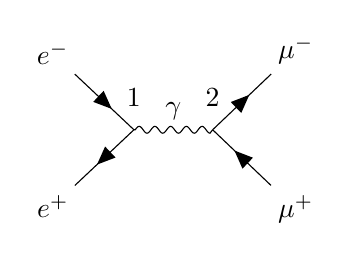
\begin{tikzpicture}[baseline={(current bounding box.center)}]
  \begin{feynman}
    %Define the positions of the vertices first.
    \vertex (a) ; %This is the first vertex
    \vertex [right= 1cm of a] (b) ; %This is the second vertex.
    %OR manually, \vertex at ($(a) + (1cm, 0)$) (b);
    %incoming arms: (the argument wihin '{\( ... \)}' is the label)
    \vertex [above  left=1cm of a] (i1) {\(e^{-}\)}; %input point 1
    \vertex [below  left=1cm of a] (i2) {\(e^{+}\)}; %input point 2
    %outgoing arms
    \vertex [above right=1cm of b] (o1) {\(\mu^{-}\)}; %output point 1
    \vertex [below right=1cm of b] (o2) {\(\mu^{+}\)}; %output point 2
    
    \diagram* {
      %This is where the lines are defined.
      %connect a and b through a boson line.
      (a) --[boson, edge label=\(\gamma\)] (b);
      %connect the incoming electrons via vertex a using fermion lines.
      %the order determines the arrow direction. Be careful!
      (i1) --[fermion] (a) --[fermion] (i2);
      %In case of fermions, the order determions the direction of arrows.
      %connect the outgoing muons via vertex b using fermion lines.
      (o2) --[fermion] (b) --[fermion] (o1);
    };
    %The diagram is complete. We can put some index number
    just above the two vertices as shown below.
    \vertex [above=0.5em of a] {\(1\)};
    %OR \vertex at ($(a) + (0, 0.5em)$) (vertex_name) {\(1)\)};
    \vertex [above=0.5em of b] {\(2\)};
  \end{feynman}
\end{tikzpicture}
\hfill
%%%%%%%%%%%%%%%%%%%%%%%%%%%%%%%%%%%%%%%%%%%%%%%%%%%%%%
%           e-mu scattering with a loop              %
%%%%%%%%%%%%%%%%%%%%%%%%%%%%%%%%%%%%%%%%%%%%%%%%%%%%%%
\begin{tikzpicture}[baseline={(current bounding box.center)}]
  \begin{feynman}
    \vertex (a) ; %This is the first vertex
    \vertex [right = 0.5cm of a ](l1); %This is where the loop begins
    \vertex [right = 1cm of l1 ](l2); %This is where the loop ends
    \vertex [right= 0.5cm of l2] (b) ; %This is the last vertex.
    %incoming arms: 
    \vertex [above  left=1cm of a] (i1) {\(e^{-}\)}; %input point 1
    \vertex [below  left=1cm of a] (i2) {\(e^{+}\)}; %input point 2
    %outgoing arms
    \vertex [above right=1cm of b] (o1) {\(\mu^{-}\)}; %output point 1
    \vertex [below right=1cm of b] (o2) {\(\mu^{+}\)}; %output point 2
    
    \diagram* { %This is where the lines are defined.
      %incoming lines:
      (i1) --[fermion2] (a) --[fermion2] (i2);
      %internal lines:
      % a is connnected to the loop
      (a) --[boson] (l1);
      %the loop between l1 and l2:
      (l1) --[fermion2, half left, edge label=\(e^-\)] (l2);
      %produces a half circle on the top half
      (l2) --[fermion2, half left, edge label=\(e^+\)] (l1);
      %produces a half circle on the bottom half
      %the loop is connected to b
      (l2) --[boson] (b);
      %outgoing lines:
      (o1) --[fermion2] (b) --[fermion2] (o2);
    };
  \end{feynman}
\end{tikzpicture}
\hfill
%%%%%%%%%%%%%%%%%%%%%%%%%%%%%%%%%%%%%%%%%%%%%%%%%%%%%%
%              gamma-gamma scattering                %
%%%%%%%%%%%%%%%%%%%%%%%%%%%%%%%%%%%%%%%%%%%%%%%%%%%%%%
\noindent
\begin{tikzpicture}[baseline={(current bounding box.center)}]
  \begin{feynman}
    \vertex (a); %first vertex of the square (top left)
    \vertex [below =1cm of a] (b); %bottom left vertex
    \vertex [right =1cm of a] (c); %top right vertex
    \vertex [right =1cm of b] (d); %bottom right vertex

    %input photons
    \vertex [above left =0.7cm of a] (i1) {\(\gamma\)};
    %photon connnected to top left vertex
    \vertex [below left =0.7cm of b] (i2) {\(\gamma\)};
    %photon connnected to bottom left vertex 
    \vertex [above right =0.7cm of c] (o1) {\(\gamma\)};
    %photon connnected to top right vertex
    \vertex [below right =0.7cm of d] (o2) {\(\gamma\)};
    %photon connnected to bottom right vertex 
    \diagram*{
      %connecting the photons to their respective vertices:
      (i1) -- [boson] (a),
      (i2) -- [boson] (b),
      (o1) -- [boson] (c),
      (o2) -- [boson] (d),
      %joining the square using fermions lines
      %continuosly going as a->c->d->b->a (clockwise)
      (a) --[fermion1] (c) --[fermion1] (d) --[fermion1] (b) --[fermion1] (a),
    };
  \end{feynman}
\end{tikzpicture}\\

\noindent
In all these diagrams, the vertex positions are defined using 'above left' and 'above right'. The following are the examples where some of the vertices are positioned manually using a co-ordinate system w.r.t another vertices. Also, I will stick to the first kind of arrow, because it looks better.\\

\noindent
\textbf{Example 2 :} A diagram with a blob and several outgoing particles, with custom positioning of the anchor points.
%%%%%%%%%%%%%%%%%%%%%%%%%%%%%%%%%%%%%%%%%%%%%%%%%%%%%%
%              gamma-gamma scattering                %
%%%%%%%%%%%%%%%%%%%%%%%%%%%%%%%%%%%%%%%%%%%%%%%%%%%%%%

\noindent
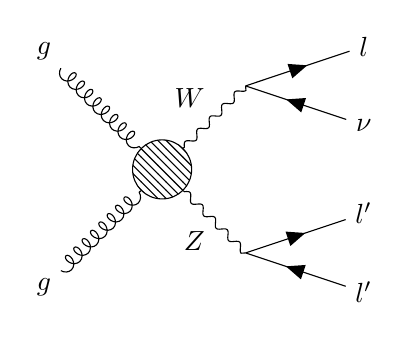
\begin{tikzpicture}[baseline={(current bounding box.center)}]
  \begin{feynman}
    \vertex [blob] (v) {\(\)}; %This is the 'blob' vertex
    %(Notice the empty label at the end). It should be there.
    %incoming points
    \vertex at($(v) + (-1.5cm, +1.5cm)$) (i1) {\(g\)};
    %Literally read it as, "the vertex i1 is at coordinates of v + (x, y)"
    \vertex at($(v) + (-1.5cm, -1.5cm)$) (i2) {\(g\)};
    %internal verices connected to the blob
    \vertex [above right =1.5cm of v] (v1);
    \vertex [below right =1.5cm of v] (v2);
    %outgoing poins
    \vertex at($(v1) + (+1.5cm, +0.5cm)$) (o1) {\(l\)};
    \vertex at($(v1) + (+1.5cm, -0.5cm)$) (o2) {\(\nu\)};
    \vertex at($(v2) + (+1.5cm, +0.5cm)$) (o3) {\(l^\prime\)};
    \vertex at($(v2) + (+1.5cm, -0.5cm)$) (o4) {\(l^\prime\)};
    \diagram*{
      %incoming lines
      (i1) --[gluon] (v);
      (i2) --[gluon]  (v);
      %internal lines
      (v) --[edge label = \(W\), boson] (v1);
      (v) --[edge label' = \(Z\), boson] (v2);
      %outgoing lines
      (o2) --[fermion] (v1) --[fermion] (o1);
      (o4) --[fermion] (v2) --[fermion] (o3);
    };
  \end{feynman}
\end{tikzpicture}\\

\noindent
\textbf{Example 3 :} A complicated diagram involving braces at several locations.\\
(The $B^0$ meson decay process as a demo.)\\

%%%%%%%%%%%%%%%%%%%%%%%%%%%%%%%%%%%%%%%%%%%%%%%%%%%%%%
%                     Meson decay                    %
%%%%%%%%%%%%%%%%%%%%%%%%%%%%%%%%%%%%%%%%%%%%%%%%%%%%%%
\noindent
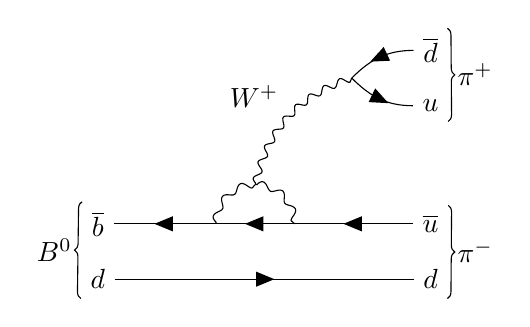
\begin{tikzpicture}[baseline={(current bounding box.center)}]
  \begin{feynman}
    \vertex (a1) {\(\overline b\)};
    \vertex[right=1.5cm of a1] (a2);
    \vertex[right=1cm of a2] (a3);
    \vertex[right=1.5cm of a3] (a4) {\(\overline u\)};
    % a1--a4 are the points on the top line
    \vertex[below=2em of a1] (b1) {\(d\)};
    \vertex[below=2em of a4] (b2) {\(d\)};
    % b1-b2 are the points on the bottom line
    %% See section 13.5 of PGF/TikZ manual
    \vertex at ($(a2)!0.5!(a3)!0.5cm!90:(a3)$) (d);
    %The other vertex at the loop is defined like this.
    %% Equivalent way to obtain (d):
    % \vertex at ($(b2)!0.5!(b3) + (0, -0.5cm)$) (d);
    \vertex[above=of a4] (c1) {\(u\)};
    \vertex[above=2em of c1] (c3) {\(\overline d\)};
    \vertex at ($(c1)!0.5!(c3) - (1cm, 0)$) (c2);
    %c1 and c3 are the output vertex, while c2 is the vertex connected to the W
    \diagram* {
      (a4) -- [fermion] (a3) -- [fermion] (a2) -- [fermion] (a1),
      (b1) -- [fermion] (b2),
      (c3) -- [fermion, out=180, in=45] (c2) -- [fermion, out=-45, in=180] (c1),
      (a2) -- [boson, quarter left] (d) -- [boson, quarter left] (a3),
      (d) -- [boson, bend left, edge label=\(W^{+}\)] (c2),
    };
    %Adding braces at the input and the output.
    \draw [decoration={brace}, decorate] (b1.south west) -- (a1.north west)
    node [pos=0.5, left] {\(B^{0}\)};
    \draw [decoration={brace}, decorate] (c3.north east) -- (c1.south east)
    node [pos=0.5, right] {\(\pi^{+}\)};
    \draw [decoration={brace}, decorate] (a4.north east) -- (b2.south east)
    node [pos=0.5, right] {\(\pi^{-}\)};
  \end{feynman}
\end{tikzpicture}\\

\vfill
\noindent
\textbf{Example 4 :} Use of colored lines and symbols.\\
(The VLL production process as a demo.)\\

%%%%%%%%%%%%%%%%%%%%%%%%%%%%%%%%%%%%%%%%%%%%%%%%%%%%%%
%                      VLL                           %
%%%%%%%%%%%%%%%%%%%%%%%%%%%%%%%%%%%%%%%%%%%%%%%%%%%%%%

\noindent
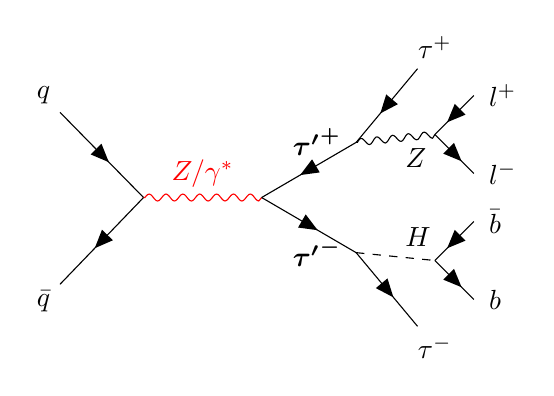
\begin{tikzpicture}[baseline={(current bounding box.center)}]
  \begin{feynman}
    \vertex (v1);
    \vertex [right =1.5cm of v1] (v2);
    %incoming points
    \vertex [above left =1.5cm of v1] (i1) {\(q\)};
    \vertex [below left =1.5cm of v1] (i2) {\(\bar{q}\)};
    %internal verices connected to the a
    \vertex at($(v2)+(1.2, +0.7)$) (b1);
    \vertex at($(v2)+(1.2, -0.7)$)(b2);
    %internal vertices connected to b1 and b2
    \vertex at($(b1)+(1.0, +0.1)$) (c1);
    \vertex at($(b2)+(1.0, -0.1)$) (c2); 
    %outgoing poins
    \vertex at($(b1) + (1.0, +1.2)$) (o1) {\(\tau^+\)};
    \vertex [above right =0.7cm of c1] (o2);
    \vertex [below right =0.7cm of c1] (o3);
    \vertex [above right =0.7cm of c2] (o4);
    \vertex [below right =0.7cm of c2] (o5);
    \vertex at($(b2) + (1.0, -1.2)$) (o6) {\(\tau^-\)};
    \diagram*{
      %incoming lines
      (i1) --[fermion] (v1) --[fermion] (i2);
      %internal lines
      (v1) --[boson, color=red, edge label = \({\color{red} Z/\gamma^*}\)] (v2);
      (b1) --[fermion] (v2) --[fermion] (b2);
      (b1) --[boson, edge label' = \(Z\)] (c1);
      (b2) --[scalar, edge label = \(H\)] (c2);
      %outgoing lines
      (o1) --[fermion] (b1);
      (o2) --[fermion] (c1) --[fermion] (o3);
      (o4) --[fermion] (c2) --[fermion] (o5);
      (b2) --[fermion] (o6);
    };
    %labels (manually putting them here because too crowded)
    %\vertex [right =0.2em of o1] (l1) {\(\tau^+\)};
    \vertex [right =0.2em of o2] (l2) {\(l^+\)};
    \vertex [right =0.2em of o3] (l3) {\(l^-\)};
    \vertex [right =0.2em of o4] (l4) {\(\bar{b}\)};
    \vertex [right =0.2em of o5] (l5) {\(b\)};
    %\vertex [right =0.2em of o6] (l6) {\(\tau^-\)};
    \vertex [left = 0.2em of b1] (tau1) {\( \boldsymbol{{\tau^{\prime}}^+} \)};
    \vertex [left = 0.2em of b2] (tau2) {\( \boldsymbol{{\tau^{\prime}}^-} \)};
  \end{feynman}
\end{tikzpicture}\\


%%%%%%%%%%%%%%%%%%%%%%%%%%%%%%%%%%%%%%%%%%%%%%%%%%%%%%
%%%%%%%%%%%%%%%%%%%%%%%%%%%%%%%%%%%%%%%%%%%%%%%%%%%%%%
% The document ends here.
\end{document}


